\documentclass[11pt]{article}
\usepackage[margin=1in]{geometry}
\usepackage{booktabs}
\usepackage{pgfplots}
\usepackage{siunitx}
\pgfplotsset{compat=1.17}
\usepackage[T1]{fontenc}
\usepackage{lmodern}

\title{Equivalence judgments and mutation scores\\for the factorial program}
\author{Generated from the collected model runs}
\date{\today}

\begin{document}
\sloppy
\maketitle

\section{Question and data}

Fourteen models judged the unit mutants of \texttt{factorial.c}. Thirteen ran through Ollama and one, \texttt{nvidia/nemotron-3-ultra-550b-a55b:free}, ran through OpenRouter. The list is \texttt{scripts/slms.txt}. The repeated provider field on the Ministral 8B line is read as provider \texttt{ollama} and model \texttt{ministral-3:8b}.

Each model has a directory \texttt{programs/factorial-<model>}. The equivalence CSV in \texttt{result/} supplies the model status of every mutant. The newest \texttt{FACTORIAL\_*.lst} report supplies the Proteum mutation score after that model's test set was executed. The files in \texttt{testset/} are the test cases exported from the model.

The hand classification marks 19 of 242 mutants equivalent: 2, 3, 5, 100, 111, 112, 123, 131, 136, 137, 167, 193, 197, 199, 200, 202, 203, 212, 231. Two of those, 167, 212, were removed by trivial compiler equivalence before a model was asked, so the models could judge 17 hand-equivalent mutants. Thirty further mutants are anomalous and were also withheld. A suggestion is a mutant whose model status is \texttt{equivalent}. Statuses \texttt{equivalent-trivial} and \texttt{anomalous} are not model suggestions.

The suggestion rate is the number of suggestions divided by the 210 mutants the model was asked to judge. Precision is the number of those suggestions that are in the hand-equivalent set, divided by the number of suggestions. The Wilson 95\% interval is reported for both proportions. Recall, reported alongside precision, is the fraction of the 17 judged hand-equivalent mutants that the model suggested. The mutation score is the value Proteum printed. It equals the mutants killed by the executed test set divided by the mutants that remain after anomalous and Proteum-equivalent mutants are removed. Unique test cases are distinct keyboard and command-line inputs in \texttt{testset/}.

\section{Equivalence suggestions}

The models suggested between 0 and 210 equivalent mutants. codegemma:2b (ollama) suggested the most, 210 (100.0\% of the mutants it judged). deepseek-coder:1.3b (ollama) suggested the fewest, 0. Figure~\ref{fig:suggestions} shows the counts, with the value printed on each bar. The rate and its Wilson interval are in Table~\ref{tab:summary} and Figure~\ref{fig:rate}.

\begin{figure}[ht]
\centering
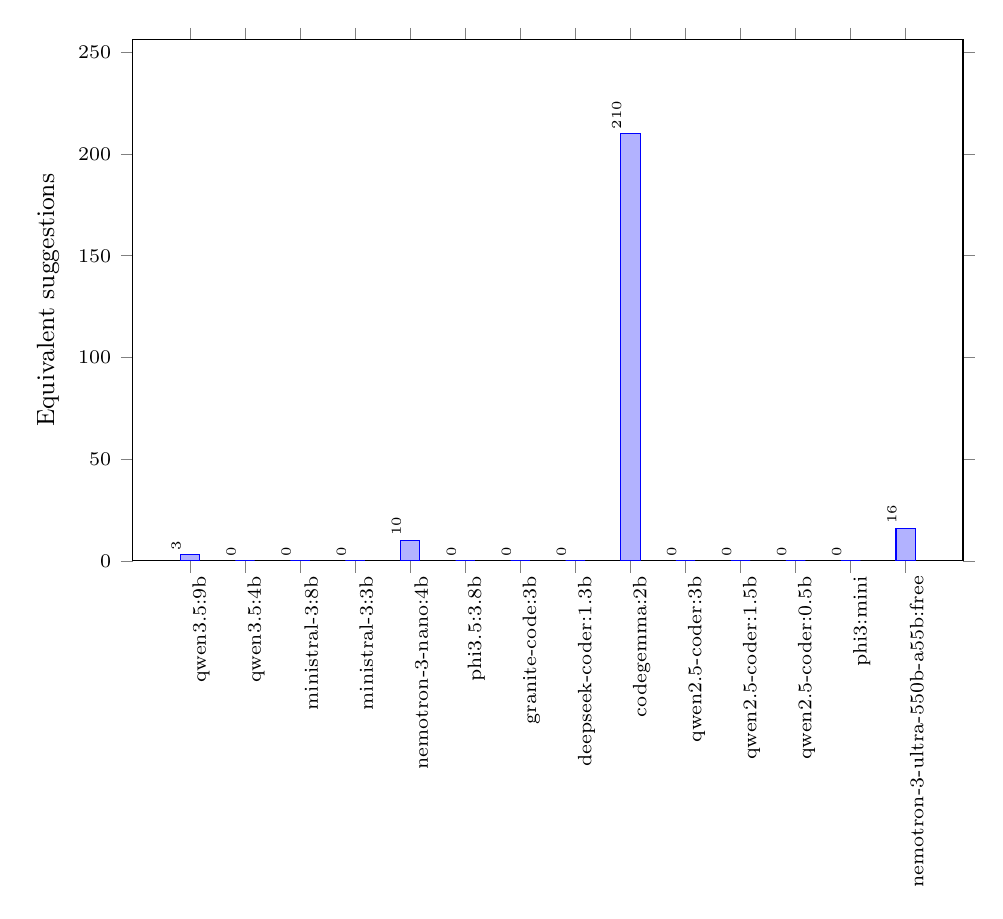
\begin{tikzpicture}
\begin{axis}[
  ybar,
  bar width=7pt,
  bar shift=0pt,
  width=\textwidth,
  height=8.2cm,
  ylabel={Equivalent suggestions},
  xtick={0,1,2,3,4,5,6,7,8,9,10,11,12,13},
  xticklabels={qwen3.5:9b,qwen3.5:4b,ministral-3:8b,ministral-3:3b,nemotron-3-nano:4b,phi3.5:3.8b,granite-code:3b,deepseek-coder:1.3b,codegemma:2b,qwen2.5-coder:3b,qwen2.5-coder:1.5b,qwen2.5-coder:0.5b,phi3:mini,nemotron-3-ultra-550b-a55b:free},
  x tick label style={rotate=90, anchor=east, font=\scriptsize, inner sep=1pt, yshift=-4pt},
  y tick label style={font=\scriptsize},
  label style={font=\small},
  ymin=0,
  ymax=256.200000,
  enlarge x limits=0.08,
  tick align=outside,
  clip=false,
]
\addplot+[bar shift=0pt] coordinates {(0,3.000000) (1,0.000000) (2,0.000000) (3,0.000000) (4,10.000000) (5,0.000000) (6,0.000000) (7,0.000000) (8,210.000000) (9,0.000000) (10,0.000000) (11,0.000000) (12,0.000000) (13,16.000000)};
\addplot[
  only marks,
  mark=none,
  bar shift=0pt,
  forget plot,
  nodes near coords,
  point meta=explicit symbolic,
  every node near coord/.append style={font=\tiny, rotate=90, anchor=west, inner sep=1.5pt, yshift=5pt, fill=white, fill opacity=0.9, text opacity=1},
] table[x=x,y=y,meta=label] {
x y label
0 3.000000 {3}
1 0.000000 {0}
2 0.000000 {0}
3 0.000000 {0}
4 10.000000 {10}
5 0.000000 {0}
6 0.000000 {0}
7 0.000000 {0}
8 210.000000 {210}
9 0.000000 {0}
10 0.000000 {0}
11 0.000000 {0}
12 0.000000 {0}
13 16.000000 {16}
};
\end{axis}
\end{tikzpicture}

\caption{Equivalent mutants suggested by each model. The number on each bar is the suggestion count.}
\label{fig:suggestions}
\end{figure}

\begin{figure}[ht]
\centering
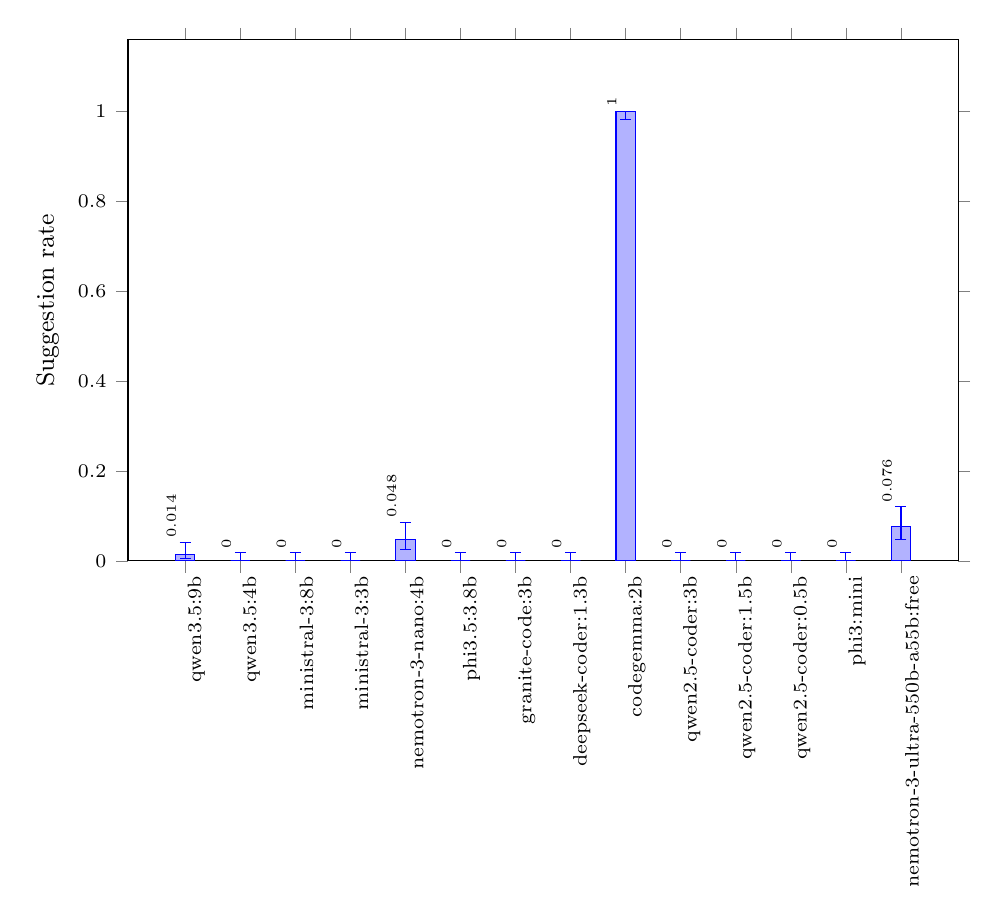
\begin{tikzpicture}
\begin{axis}[
  ybar,
  bar width=7pt,
  bar shift=0pt,
  width=\textwidth,
  height=8.2cm,
  ylabel={Suggestion rate},
  xtick={0,1,2,3,4,5,6,7,8,9,10,11,12,13},
  xticklabels={qwen3.5:9b,qwen3.5:4b,ministral-3:8b,ministral-3:3b,nemotron-3-nano:4b,phi3.5:3.8b,granite-code:3b,deepseek-coder:1.3b,codegemma:2b,qwen2.5-coder:3b,qwen2.5-coder:1.5b,qwen2.5-coder:0.5b,phi3:mini,nemotron-3-ultra-550b-a55b:free},
  x tick label style={rotate=90, anchor=east, font=\scriptsize, inner sep=1pt, yshift=-4pt},
  y tick label style={font=\scriptsize},
  label style={font=\small},
  ymin=0,
  ymax=1.160000,
  enlarge x limits=0.08,
  tick align=outside,
  clip=false,
]
\addplot+[
  bar shift=0pt,
  error bars/.cd,
  y dir=both,
  y explicit,
  error bar style={thin}
] table[x=x,y=y,y error minus=minus,y error plus=plus] {
x y minus plus
0 0.014286 0.009416 0.026866
1 0.000000 0.000000 0.017964
2 0.000000 0.000000 0.017964
3 0.000000 0.000000 0.017964
4 0.047619 0.021551 0.037804
5 0.000000 0.000000 0.017964
6 0.000000 0.000000 0.017964
7 0.000000 0.000000 0.017964
8 1.000000 0.017964 0.000000
9 0.000000 0.000000 0.017964
10 0.000000 0.000000 0.017964
11 0.000000 0.000000 0.017964
12 0.000000 0.000000 0.017964
13 0.076190 0.028751 0.043978
};
\addplot[
  only marks,
  mark=none,
  bar shift=0pt,
  forget plot,
  nodes near coords,
  point meta=explicit symbolic,
  every node near coord/.append style={font=\tiny, rotate=90, anchor=west, inner sep=1.5pt, yshift=5pt, fill=white, fill opacity=0.9, text opacity=1},
] table[x=x,y=y,meta=label] {
x y label
0 0.041152 {0.014}
1 0.017964 {0}
2 0.017964 {0}
3 0.017964 {0}
4 0.085423 {0.048}
5 0.017964 {0}
6 0.017964 {0}
7 0.017964 {0}
8 1.000000 {1}
9 0.017964 {0}
10 0.017964 {0}
11 0.017964 {0}
12 0.017964 {0}
13 0.120168 {0.076}
};
\end{axis}
\end{tikzpicture}

\caption{Suggestion rate among the mutants submitted to the model. The number on each bar is the rate. The intervals are 95\% Wilson intervals, and each number sits above its interval.}
\label{fig:rate}
\end{figure}

\section{Precision against the hand classification}

The highest precision is 100.0\%, shared by nemotron-3-ultra-550b-a55b:free (openrouter) (16 of 16, recall 94.1\%); qwen3.5:9b (ollama) (3 of 3, recall 17.6\%). Precision is undefined for qwen3.5:4b, ministral-3:8b, ministral-3:3b, phi3.5:3.8b, granite-code:3b, deepseek-coder:1.3b, qwen2.5-coder:3b, qwen2.5-coder:1.5b, qwen2.5-coder:0.5b, phi3:mini because those models suggested no equivalent mutant.

A high suggestion count is not a high precision. A model that calls every judged mutant equivalent records a suggestion rate of 100\% and a precision equal to the prevalence of hand-equivalent mutants in that judged set. Figure~\ref{fig:precision} shows the defined precisions.

\begin{figure}[ht]
\centering
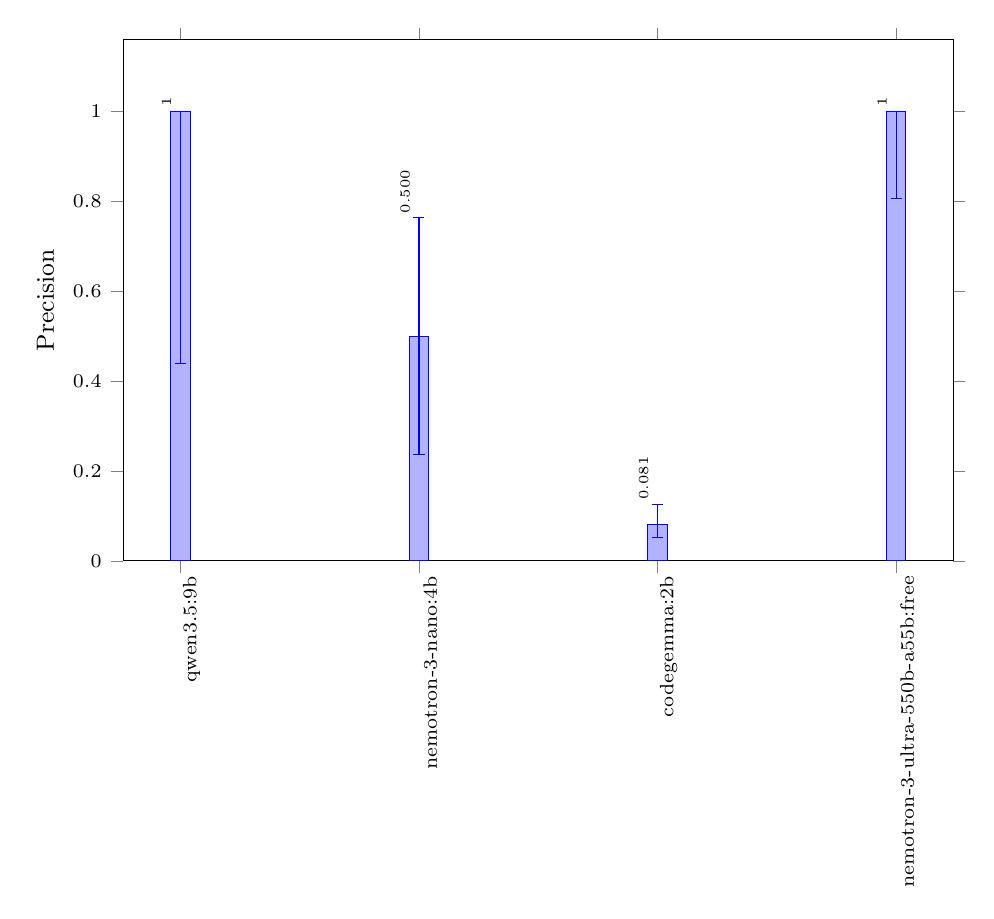
\begin{tikzpicture}
\begin{axis}[
  ybar,
  bar width=7pt,
  bar shift=0pt,
  width=\textwidth,
  height=8.2cm,
  ylabel={Precision},
  xtick={0,1,2,3},
  xticklabels={qwen3.5:9b,nemotron-3-nano:4b,codegemma:2b,nemotron-3-ultra-550b-a55b:free},
  x tick label style={rotate=90, anchor=east, font=\scriptsize, inner sep=1pt, yshift=-4pt},
  y tick label style={font=\scriptsize},
  label style={font=\small},
  ymin=0,
  ymax=1.160000,
  enlarge x limits=0.08,
  tick align=outside,
  clip=false,
]
\addplot+[
  bar shift=0pt,
  error bars/.cd,
  y dir=both,
  y explicit,
  error bar style={thin}
] table[x=x,y=y,y error minus=minus,y error plus=plus] {
x y minus plus
0 1.000000 0.561497 0.000000
1 0.500000 0.263407 0.263407
2 0.080952 0.029797 0.044853
3 1.000000 0.193608 0.000000
};
\addplot[
  only marks,
  mark=none,
  bar shift=0pt,
  forget plot,
  nodes near coords,
  point meta=explicit symbolic,
  every node near coord/.append style={font=\tiny, rotate=90, anchor=west, inner sep=1.5pt, yshift=5pt, fill=white, fill opacity=0.9, text opacity=1},
] table[x=x,y=y,meta=label] {
x y label
0 1.000000 {1}
1 0.763407 {0.500}
2 0.125805 {0.081}
3 1.000000 {1}
};
\end{axis}
\end{tikzpicture}

\caption{Precision of equivalent suggestions against the hand classification. The number on each bar is the precision. The intervals are 95\% Wilson intervals. Models with no suggestions are omitted.}
\label{fig:precision}
\end{figure}

\section{Mutation score}

After each model's test set was executed, Proteum's mutation score ranged from 0.243 to 0.929. The highest score is ministral-3:8b (ollama), with 15 mutants still alive. Figure~\ref{fig:score} orders the models by that score. The score already excludes the 30 anomalous mutants and the 2 mutants Proteum holds as equivalent, so it is computed from the mutants the test set killed.

\begin{figure}[ht]
\centering
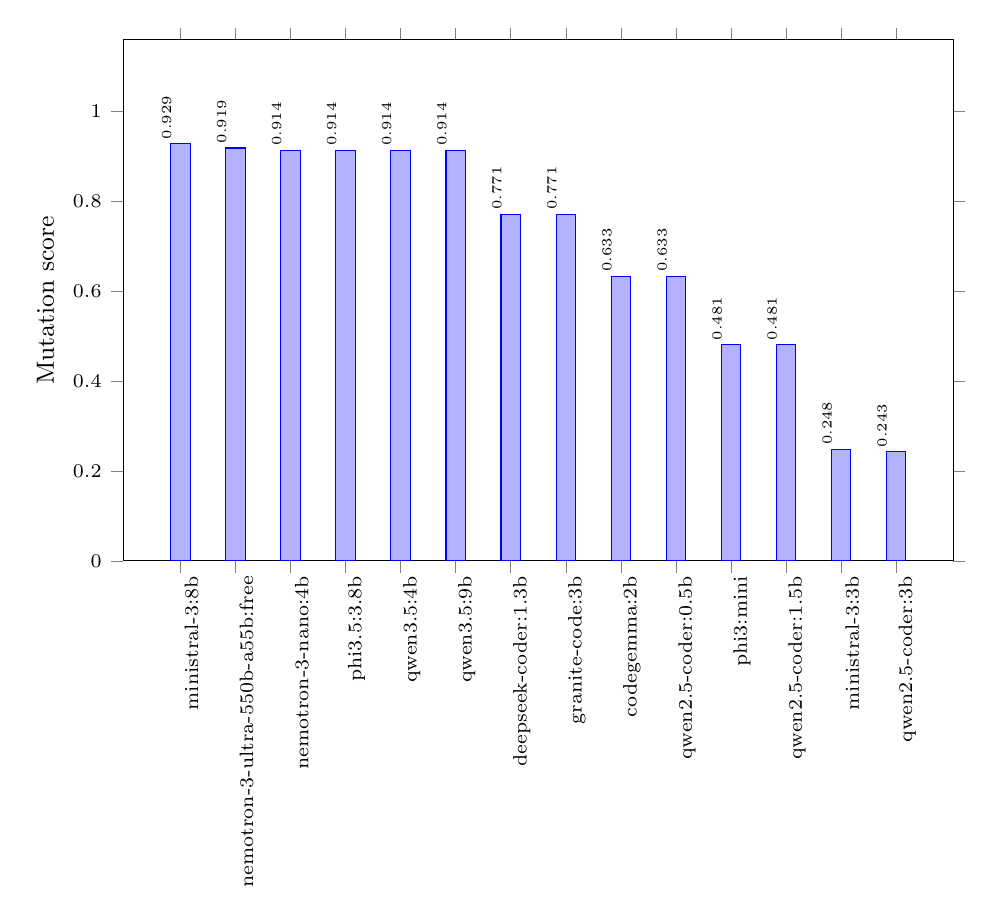
\begin{tikzpicture}
\begin{axis}[
  ybar,
  bar width=7pt,
  bar shift=0pt,
  width=\textwidth,
  height=8.2cm,
  ylabel={Mutation score},
  xtick={0,1,2,3,4,5,6,7,8,9,10,11,12,13},
  xticklabels={ministral-3:8b,nemotron-3-ultra-550b-a55b:free,nemotron-3-nano:4b,phi3.5:3.8b,qwen3.5:4b,qwen3.5:9b,deepseek-coder:1.3b,granite-code:3b,codegemma:2b,qwen2.5-coder:0.5b,phi3:mini,qwen2.5-coder:1.5b,ministral-3:3b,qwen2.5-coder:3b},
  x tick label style={rotate=90, anchor=east, font=\scriptsize, inner sep=1pt, yshift=-4pt},
  y tick label style={font=\scriptsize},
  label style={font=\small},
  ymin=0,
  ymax=1.160000,
  enlarge x limits=0.08,
  tick align=outside,
  clip=false,
]
\addplot+[bar shift=0pt] coordinates {(0,0.928571) (1,0.919048) (2,0.914286) (3,0.914286) (4,0.914286) (5,0.914286) (6,0.771429) (7,0.771429) (8,0.633333) (9,0.633333) (10,0.480952) (11,0.480952) (12,0.247619) (13,0.242857)};
\addplot[
  only marks,
  mark=none,
  bar shift=0pt,
  forget plot,
  nodes near coords,
  point meta=explicit symbolic,
  every node near coord/.append style={font=\tiny, rotate=90, anchor=west, inner sep=1.5pt, yshift=5pt, fill=white, fill opacity=0.9, text opacity=1},
] table[x=x,y=y,meta=label] {
x y label
0 0.928571 {0.929}
1 0.919048 {0.919}
2 0.914286 {0.914}
3 0.914286 {0.914}
4 0.914286 {0.914}
5 0.914286 {0.914}
6 0.771429 {0.771}
7 0.771429 {0.771}
8 0.633333 {0.633}
9 0.633333 {0.633}
10 0.480952 {0.481}
11 0.480952 {0.481}
12 0.247619 {0.248}
13 0.242857 {0.243}
};
\end{axis}
\end{tikzpicture}

\caption{Proteum mutation score after executing the test set generated by each model. The number on each bar is the score.}
\label{fig:score}
\end{figure}

\subsection{Alive mutants that separate the two highest scores}

ministral-3:8b (ollama) left 15 mutants alive: 2, 3, 5, 100, 111, 112, 123, 131, 136, 137, 193, 199, 200, 202, and 231. nemotron-3-ultra-550b-a55b:free (openrouter) left those same 15 alive and also left 197 and 203 alive. Both extra mutants are operator \texttt{u-VDTR}. They replace an operand with \texttt{TRAP\_ON\_ZERO} applied to \texttt{fat}: mutant 197 in the multiplication, and mutant 203 in the printed value. The two extra kills are the whole gap between the scores 0.929 and 0.919.

Ministral's test set killed both. Proteum records the killing input as test case 6, which is test case \#7 in the test-case report. The keyboard input is 42. For that input the factorial overflows a 32-bit \texttt{int} and the original program prints 0, so \texttt{TRAP\_ON\_ZERO} fires. A test that produces this difference shows that mutants 197 and 203 differ from the original.

An overflowing factorial prints 0 when the factorial contains at least 32 factors of two. Input 12 still fits and prints 479001600. Inputs 13 through 33 overflow and print a nonzero wrapped value, including 1932053504 for 13 and $-2147483648$ for 32 and 33. From 34 upward, including 42, the program prints 0.

The hand file lists 197 and 203 as equivalent, together with the 15 mutants that stayed alive for both models. The precision and recall in this report follow that file. Under it, the OpenRouter model suggested both mutants were equivalent, so both count as true positives. The killing input shows those two hand labels disagree with the execution. Mutants 167 and 212 are also hand-equivalent, and they are absent from both alive sets because Proteum already holds them as the two trivial equivalents. The OpenRouter session was later updated so the 17 mutants above are marked equivalent; the score in Figure~\ref{fig:score} is the score from the report written when those 17 were still alive.

\section{Unique test cases}

The exported test sets contain between 1 and 9 distinct inputs. nemotron-3-nano:4b (ollama) produced the largest set. Figure~\ref{fig:tests} shows the counts, with the value printed on each bar. Across the 14 models, the Spearman rank correlation between the number of unique test cases and the mutation score is 0.763. Figure~\ref{fig:scatter} plots the two quantities. The association is descriptive: each model contributes one pair, and the test inputs are not a random sample.

\begin{figure}[ht]
\centering
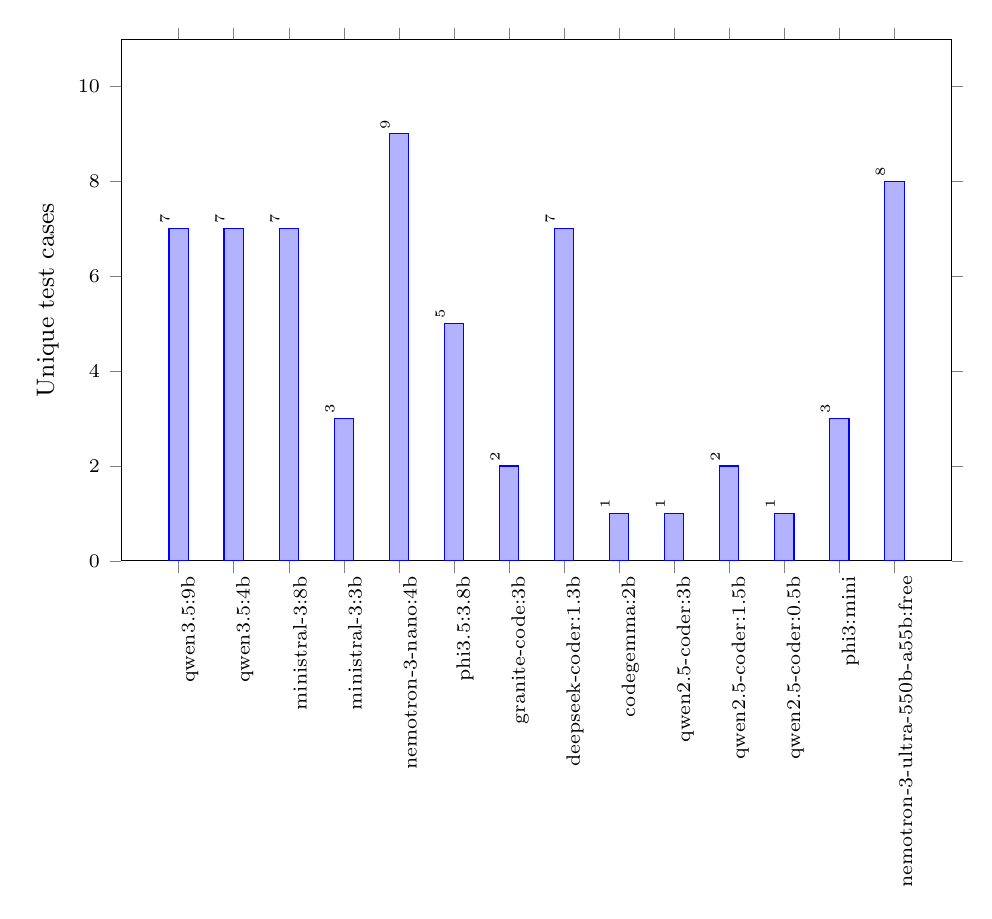
\begin{tikzpicture}
\begin{axis}[
  ybar,
  bar width=7pt,
  bar shift=0pt,
  width=\textwidth,
  height=8.2cm,
  ylabel={Unique test cases},
  xtick={0,1,2,3,4,5,6,7,8,9,10,11,12,13},
  xticklabels={qwen3.5:9b,qwen3.5:4b,ministral-3:8b,ministral-3:3b,nemotron-3-nano:4b,phi3.5:3.8b,granite-code:3b,deepseek-coder:1.3b,codegemma:2b,qwen2.5-coder:3b,qwen2.5-coder:1.5b,qwen2.5-coder:0.5b,phi3:mini,nemotron-3-ultra-550b-a55b:free},
  x tick label style={rotate=90, anchor=east, font=\scriptsize, inner sep=1pt, yshift=-4pt},
  y tick label style={font=\scriptsize},
  label style={font=\small},
  ymin=0,
  ymax=10.980000,
  enlarge x limits=0.08,
  tick align=outside,
  clip=false,
]
\addplot+[bar shift=0pt] coordinates {(0,7.000000) (1,7.000000) (2,7.000000) (3,3.000000) (4,9.000000) (5,5.000000) (6,2.000000) (7,7.000000) (8,1.000000) (9,1.000000) (10,2.000000) (11,1.000000) (12,3.000000) (13,8.000000)};
\addplot[
  only marks,
  mark=none,
  bar shift=0pt,
  forget plot,
  nodes near coords,
  point meta=explicit symbolic,
  every node near coord/.append style={font=\tiny, rotate=90, anchor=west, inner sep=1.5pt, yshift=5pt, fill=white, fill opacity=0.9, text opacity=1},
] table[x=x,y=y,meta=label] {
x y label
0 7.000000 {7}
1 7.000000 {7}
2 7.000000 {7}
3 3.000000 {3}
4 9.000000 {9}
5 5.000000 {5}
6 2.000000 {2}
7 7.000000 {7}
8 1.000000 {1}
9 1.000000 {1}
10 2.000000 {2}
11 1.000000 {1}
12 3.000000 {3}
13 8.000000 {8}
};
\end{axis}
\end{tikzpicture}

\caption{Distinct test inputs exported for each model. The number on each bar is the count.}
\label{fig:tests}
\end{figure}

\begin{figure}[ht]
\centering
\begin{tikzpicture}
\begin{axis}[
  width=0.82\textwidth,
  height=7.2cm,
  xlabel={Unique test cases},
  ylabel={Mutation score},
  xmin=-0.4,
  ymin=0,
  ymax=1,
  tick align=outside,
  label style={font=\small},
  tick label style={font=\scriptsize},
  only marks,
  mark size=1.8pt,
]
\addplot coordinates {(7,0.914286) (7,0.914286) (7,0.928571) (3,0.247619) (9,0.914286) (5,0.914286) (2,0.771429) (7,0.771429) (1,0.633333) (1,0.242857) (2,0.480952) (1,0.633333) (3,0.480952) (8,0.919048)};
\end{axis}
\end{tikzpicture}

\caption{Mutation score against the number of unique test cases.}
\label{fig:scatter}
\end{figure}

\section{Summary}

Table~\ref{tab:summary} collects the four quantities. Suggestions and the suggestion rate answer how many equivalent mutants each model detected. True positives, false positives, and precision answer how many of those detections match the hand classification. The mutation score is the Proteum score after the model's test set ran. Tests is the number of unique inputs in that test set.

\begin{table}[ht]
\centering
\caption{Equivalence suggestions, precision, mutation score, and unique tests. Rate and precision are percentages.}
\label{tab:summary}
\scriptsize
\begin{tabular}{@{}llrrrrrrr@{}}
\toprule
Provider & Model & Suggestions & Rate & TP & FP & Precision & Score & Tests \\
\midrule
ollama & qwen3.5:9b & 3 & 1.4\% & 3 & 0 & 100.0\% & 0.914 & 7 \\
ollama & qwen3.5:4b & 0 & 0.0\% & 0 & 0 & NA & 0.914 & 7 \\
ollama & ministral-3:8b & 0 & 0.0\% & 0 & 0 & NA & 0.929 & 7 \\
ollama & ministral-3:3b & 0 & 0.0\% & 0 & 0 & NA & 0.248 & 3 \\
ollama & nemotron-3-nano:4b & 10 & 4.8\% & 5 & 5 & 50.0\% & 0.914 & 9 \\
ollama & phi3.5:3.8b & 0 & 0.0\% & 0 & 0 & NA & 0.914 & 5 \\
ollama & granite-code:3b & 0 & 0.0\% & 0 & 0 & NA & 0.771 & 2 \\
ollama & deepseek-coder:1.3b & 0 & 0.0\% & 0 & 0 & NA & 0.771 & 7 \\
ollama & codegemma:2b & 210 & 100.0\% & 17 & 193 & 8.1\% & 0.633 & 1 \\
ollama & qwen2.5-coder:3b & 0 & 0.0\% & 0 & 0 & NA & 0.243 & 1 \\
ollama & qwen2.5-coder:1.5b & 0 & 0.0\% & 0 & 0 & NA & 0.481 & 2 \\
ollama & qwen2.5-coder:0.5b & 0 & 0.0\% & 0 & 0 & NA & 0.633 & 1 \\
ollama & phi3:mini & 0 & 0.0\% & 0 & 0 & NA & 0.481 & 3 \\
openrouter & nemotron-3-ultra-550b-a55b:free & 16 & 7.6\% & 16 & 0 & 100.0\% & 0.919 & 8 \\
\bottomrule
\end{tabular}
\end{table}

\appendix
\section{Reproducing the tables}

From the repository root:

\begin{verbatim}
python3 analysis/factorial-models/analyze_models.py
Rscript analysis/factorial-models/analyze_models.R
cd analysis/factorial-models && pdflatex report.tex
\end{verbatim}

The Python script writes the CSV files in \texttt{data/}, the TikZ figures in \texttt{figures/}, and this report. The R script reads \texttt{data/model-summary.csv} and writes the same Spearman correlation.

\end{document}
